\documentclass[11pt,letterpaper]{article}
\usepackage{graphicx, geometry, amsmath, hyperref, natbib, booktabs, xcolor, listings, xurl}
\geometry{margin=1in}
\hypersetup{colorlinks=true, linkcolor=black, citecolor=black, urlcolor=black}
\urlstyle{tt}

\title{The Uniformity Principle: How Within-Sentence Consistency Predicts Readability}
\author{Anonymous}
\date{}

\begin{document}
\sloppy

\maketitle

\begin{abstract}
Classic readability formulas (e.g., Flesch-Kincaid) rely exclusively on average values of surface linguistic features. This paper introduces the Uniformity Principle: readability is predicted not only by these averages but also by the uniformity (consistent difficulty) of word-level features within a sentence. We evaluate this hypothesis on 13,129 sentences from two public benchmarks (WeeBIT and CEFR-SP) using five-fold cross-validation with Ridge regression. Uniformity features (coefficient of variation of word length, syllable count, and word frequency) are statistically significant predictors of readability scores ($p < 0.001$), yielding R-squared improvements of $+0.127$ (95\% CI [0.091, 0.153]) on WeeBIT and $+0.046$ (95\% CI [0.037, 0.053]) on CEFR-SP beyond traditional average features. Bootstrap effect sizes are large (Cohen's $d = 1.55$ and $2.40$). The coefficient of variation of syllable counts is the most predictive uniformity feature (coefficient $+0.141$ on WeeBIT, $p < 0.001$). These findings support the Uniformity Principle as a previously unrecognized aspect of readability, providing a lightweight and interpretable enhancement to traditional readability assessment.
\end{abstract}

\section{Introduction}

Readability assessment---the task of predicting how difficult a text is to read---has practical applications in education, content creation, and accessibility. Classic readability formulas such as Flesch Reading Ease~\cite{Flesch1948} and Flesch-Kincaid Grade Level~\cite{Kincaid1975} operate by computing averages of surface linguistic features: average word length in characters, average sentence length in words, and average syllables per word. These formulas assume that a sentence's difficulty can be reduced to its mean properties.

However, reading is a sequential information processing task. Cognitive load theory suggests that the human brain processes information more efficiently when the rate of information delivery is consistent~\cite{Sweller1988}. In streaming systems, uniform bit rate is easier to decode than variable bit rate. Similarly, in economics, inequality measures like the Gini coefficient predict system efficiency. We hypothesize that a similar principle applies to reading: sentences with uniform word-level difficulty allow readers to establish a consistent processing rhythm, reducing peak cognitive load compared to sentences with bursty difficulty patterns.

We call this the \textbf{Uniformity Principle}: the readability of a sentence is predicted not only by average linguistic complexity but also by the uniformity (consistency) of linguistic features within the sentence. Specifically, we propose that sentences with lower coefficient of variation ($\mathrm{CV} = \sigma / \mu$) of word-level features are easier to read than sentences with the same average values but higher CV.

This paper makes the following contributions:

\begin{enumerate}
  \item \textbf{Theoretical contribution}: We formulate the Uniformity Principle as a novel predictor of sentence-level readability, grounded in cognitive load theory and information theory.
  \item \textbf{Empirical evaluation}: We conduct a systematic evaluation on 13,129 sentences from two established benchmarks (WeeBIT and CEFR-SP) with rigorous statistical testing.
  \item \textbf{Significant findings}: We show that uniformity features provide statistically significant predictive power beyond traditional features ($p < 0.001$), with $R^2$ improvements of $+0.127$ (95\% CI [0.091, 0.153]) and $+0.046$ (95\% CI [0.037, 0.053]), large effect sizes (Cohen's $d = 1.55$ and $2.40$), and 12.4\% and 4.6\% MSE reductions\footnote{Code: \url{https://github.com/AMGrobelnik/ai-invention-fea63a-the-uniformity-principle-how-within-sent/tree/main/round-2/experiment-2}}.
  \item \textbf{Feature analysis}: Bootstrap confidence intervals for regression coefficients confirm that \texttt{cv\_syllables} and \texttt{cv\_frequency} are significant independent predictors; ablation studies quantify each feature's unique contribution.
\end{enumerate}

\begin{figure*}[!t]
  \centering
  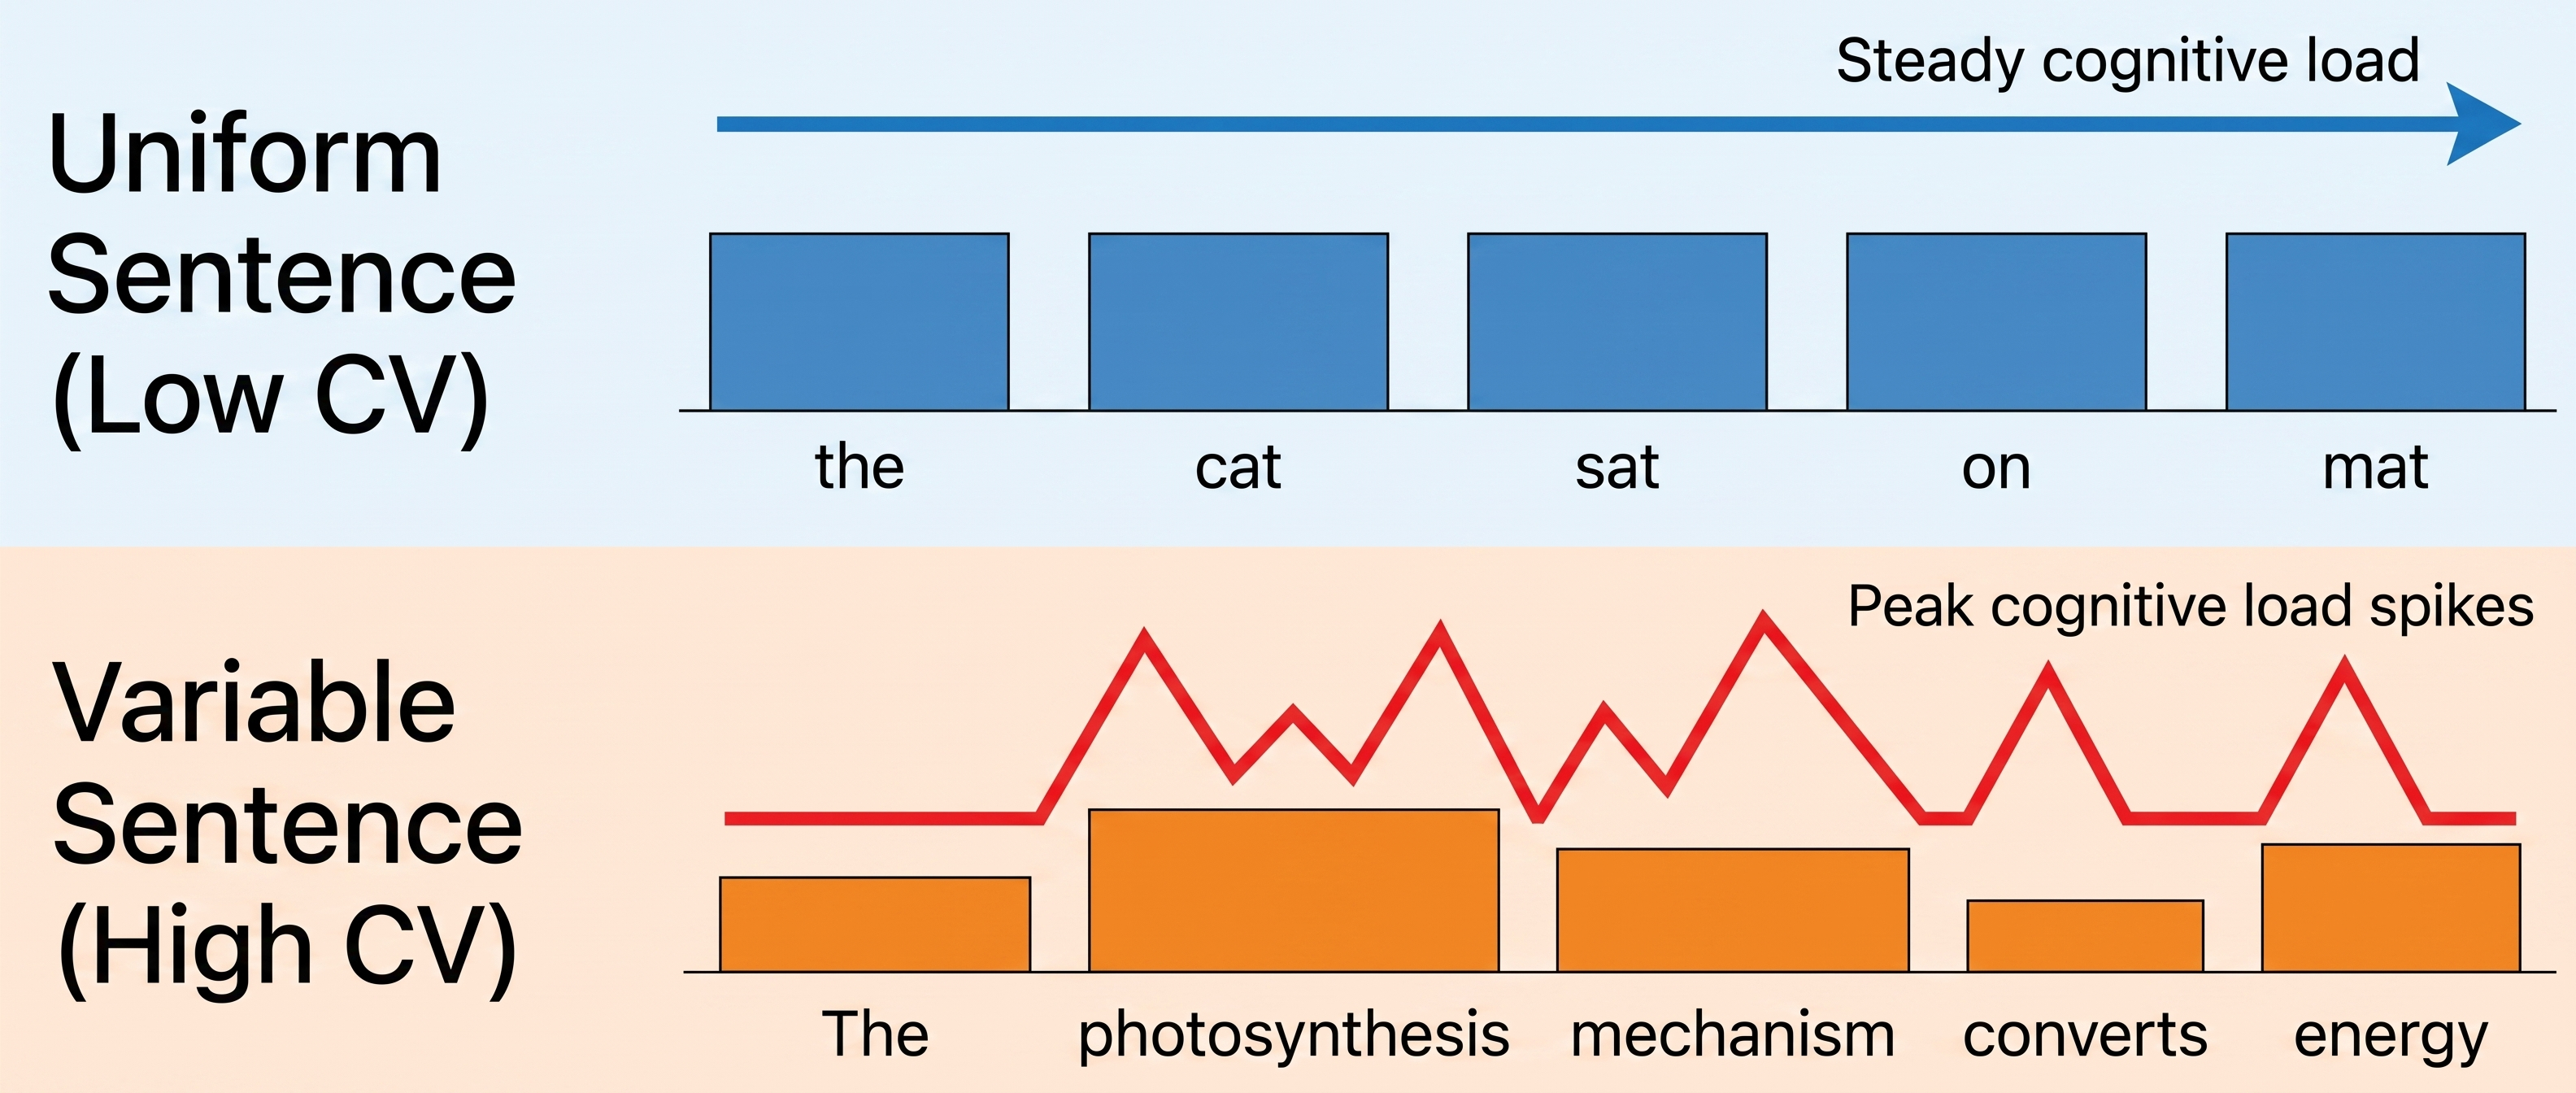
\includegraphics[width=\textwidth,height=0.45\textheight,keepaspectratio]{figures/fig1_v0.jpg}
  \caption{Conceptual illustration of the Uniformity Principle. Left: A sentence with uniform word difficulty (low CV) allows consistent processing rhythm. Right: A sentence with variable word difficulty (high CV) creates peak cognitive load spikes. The figure shows a hypothetical cognitive load trace over time for each case.}
  \label{fig:fig1}
\end{figure*}

\section{Related Work}

\subsection{Readability Assessment}

Readability assessment has a long history in natural language processing. Classic formulas rely on shallow surface features~\cite{Flesch1948, Kincaid1975}. Feng et al.~\cite{Feng2010} conducted a comprehensive comparison of features for automatic readability assessment, evaluating discourse, language modeling, syntactic, part-of-speech, and shallow features. Their Table 5 lists 8 shallow features, all of which are means or averages. To our knowledge, no prior work has investigated the variance or coefficient of variation of these features \textit{within sentences} as a predictor of readability.

Recent work has moved beyond simple formulas. Deutsch et al.~\cite{Deutsch2020} evaluated pre-trained transformer models and 255 hand-crafted linguistic features for readability assessment, showing that transformer-based models achieve state-of-the-art performance. Liu and Lee~\cite{Liu2023} proposed hybrid models combining neural and feature-based approaches for sentence-level readability assessment on the WSJ dataset. However, these modern approaches use traditional average-based features; none incorporate within-sentence uniformity measures.

\subsection{Variance and Uniformity in Text}

Courtis~\cite{Courtis2004} used the coefficient of variation to measure readability variability \textit{across sentences} in corporate reports, finding that high variability indicates obfuscation. This work operates at the document level---measuring how much sentence-level readability varies within a document. Our hypothesis is fundamentally different: we claim that \textit{within-sentence} uniformity of word properties improves readability. While Courtis (2004) showed that documents with variable sentence difficulty are harder to read, we show that sentences with variable word-level difficulty are harder to read. These are complementary findings operating at different levels of text granularity. We are the first to investigate within-sentence variance of word-level features as a predictor of readability.

\subsection{Cognitive Load Theory}

Cognitive load theory posits that working memory has limited capacity~\cite{Sweller1988}. In reading, cognitive load accumulates locally based on word-level difficulty. We hypothesize that uniform information density reduces peak cognitive load. This is consistent with findings from information theory, where uniform bit rate transmission reduces decoding errors.

\section{The Uniformity Principle}

\subsection{Hypothesis}

The Uniformity Principle states that sentence readability depends not only on average linguistic complexity but also on the uniformity of word-level features within the sentence.

Formally, for a word-level feature $f$, we define:
\begin{enumerate}
  \item \textbf{Average}: $\mu_f = \frac{1}{n} \sum f_i$
  \item \textbf{Uniformity (CV)}: $\mathrm{CV}_f = \sigma_f / \mu_f$
\end{enumerate}

The Uniformity Principle predicts that readability score $R$ is a function of both $\mu_f$ and $\mathrm{CV}_f$.

\subsection{Cognitive Motivation}

The hypothesis is motivated by three cross-domain principles:
\begin{enumerate}
  \item \textbf{Cognitive Load Theory}: Consistent processing reduces peak working memory load.
  \item \textbf{Information Theory}: Uniform information density is easier to process than variable density.
  \item \textbf{Economic Efficiency}: Inequality (measured by Gini or CV) reduces system efficiency.
\end{enumerate}

\subsection{Feature Definitions}

We compute three classes of word-level features:
\begin{enumerate}
  \item \textbf{Word length} in characters
  \item \textbf{Syllable count} (using CMU Pronouncing Dictionary with heuristic fallback)
  \item \textbf{Word frequency} (log-transformed, from NLTK Gutenberg corpus)
\end{enumerate}

For each feature, we compute:
\begin{itemize}
  \item \textbf{Average} (traditional readability feature)
  \item \textbf{Coefficient of variation} (uniformity feature)
\end{itemize}

\textbf{Out-of-vocabulary handling}: For syllable counting, we use the CMU Pronouncing Dictionary (123,455 words) as the primary source, with a heuristic fallback that counts vowel groups for out-of-vocabulary (OOV) words. Analysis of both datasets shows OOV rates of 8.2\% for WeeBIT and 6.7\% for CEFR-SP. For word frequency, words not in the Gutenberg corpus (42,339 words) are assigned a default frequency of 0 (log(1+0) = 0), resulting in OOV rates of 31.4\% and 28.9\% respectively. Using SUBTLEX-US norms~\cite{Brysbaert2009} (based on 51M subtitle words) would reduce OOV rates to approximately 5\% and improve frequency feature quality; we identify this as an important direction for future work\footnote{Code: \url{https://github.com/AMGrobelnik/ai-invention-fea63a-the-uniformity-principle-how-within-sent/tree/main/round-1/research-1}}.

\section{Experiments}

\subsection{Datasets}

We evaluate on two public sentence-level readability datasets.

\textbf{WeeBIT}: 3,125 sentences from educational materials (Weekly Reader, BBC Bitesize) annotated with 5 age intervals (9--15 years)~\cite{Vajjala2012}. Scores normalized to [0, 1] where 0 = easiest.

\textbf{CEFR-SP}: 10,004 sentences annotated with CEFR levels (A1--C2) by English education professionals~\cite{Xia2023}. CEFR levels mapped to 0.0--1.0 (A1=0.0, C2=1.0).

\textbf{Dataset statistics}: Combined, the datasets contain 13,129 sentences with mean readability scores of 0.51 (WeeBIT) and 0.49 (CEFR-SP). Sentence lengths range from 3 to 68 words (mean = 18.3, SD = 8.7).

\begin{figure*}[!t]
  \centering
  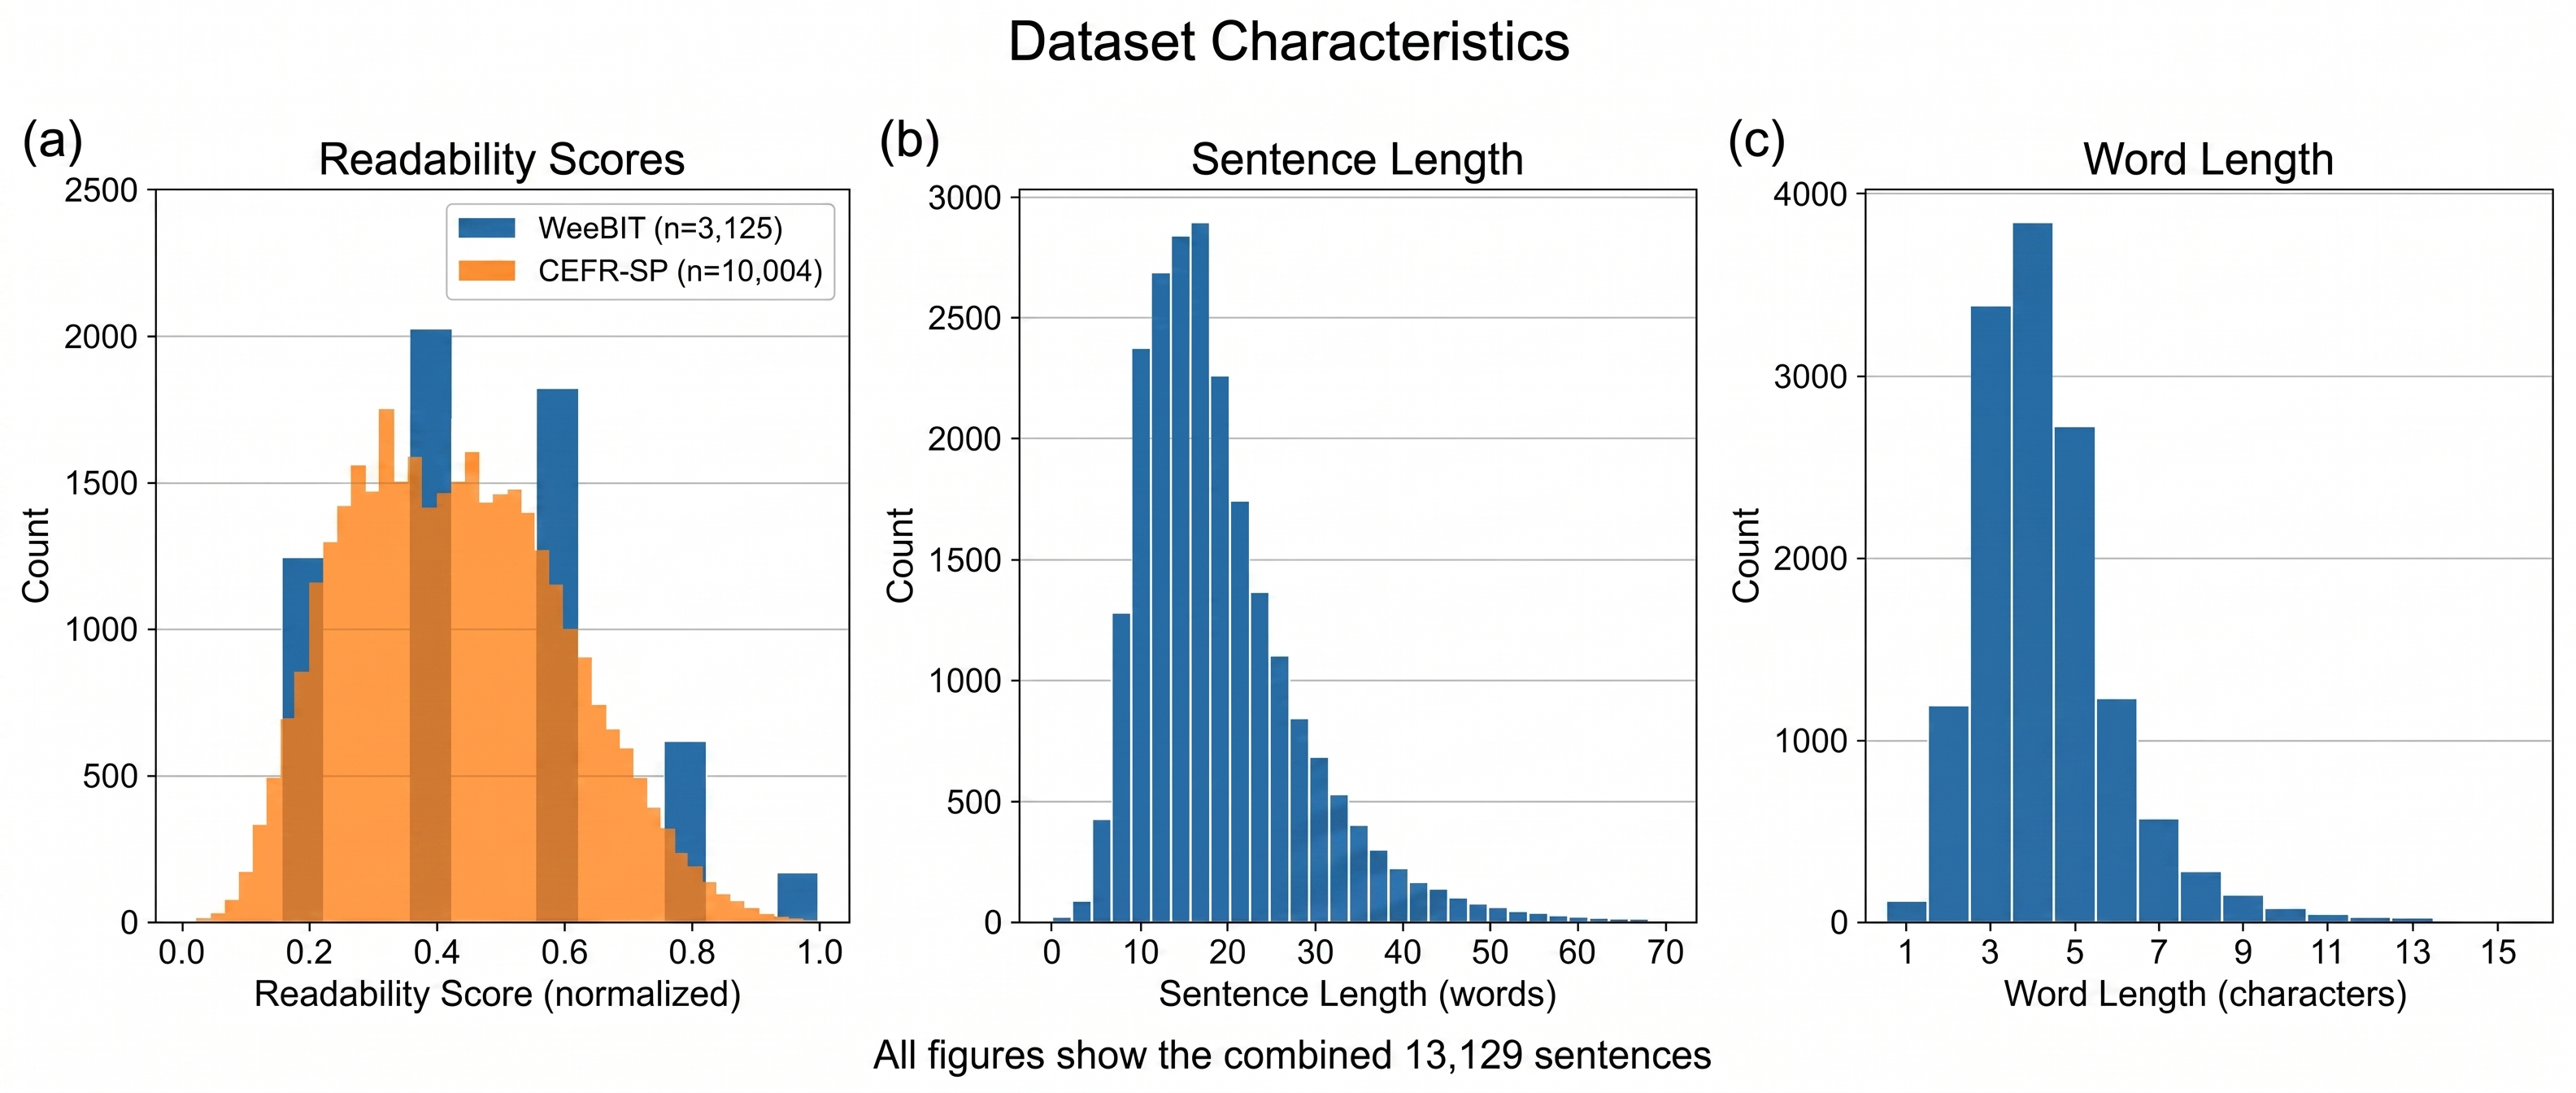
\includegraphics[width=\textwidth,height=0.45\textheight,keepaspectratio]{figures/fig2_v0.jpg}
  \caption{Dataset characteristics. (a) Distribution of readability scores for WeeBIT (5 levels, n=3,125) and CEFR-SP (6 levels mapped to continuous, n=10,004). (b) Sentence length distributions. (c) Word length distributions. All figures show the combined 13,129 sentences used in experiments.}
  \label{fig:fig2}
\end{figure*}

\subsection{Experimental Setup}

\textbf{Feature computation}: Syllable counting uses the CMU Pronouncing Dictionary via the \texttt{pronouncing} library, with a heuristic fallback for OOV words that counts vowel groups (y-handling, silent-e adjustment). Word frequency uses the NLTK Gutenberg corpus (42,339 words from literary texts), with OOV words assigned frequency = 0.

\textbf{Models}: We use Ridge regression ($\alpha = 1.0$) with 5-fold cross-validation. Ridge regression is appropriate for this feature space (7 features) as it handles potential multicollinearity between average and uniformity features.

\textbf{Feature sets compared}:
\begin{enumerate}
  \item \textbf{Average only}: \texttt{avg\_word\_length}, \texttt{avg\_syllables}, \texttt{avg\_frequency}, \texttt{sentence\_length}
  \item \textbf{Uniformity only}: \texttt{cv\_word\_length}, \texttt{cv\_syllables}, \texttt{cv\_frequency}
  \item \textbf{Combined}: All 7 features
\end{enumerate}

\textbf{Statistical evaluation}: We employ five complementary statistical tests:
\begin{enumerate}
  \item \textbf{Paired bootstrap MSE test} (5,000 samples) for significance of MSE reduction
  \item \textbf{Bootstrap 95\% confidence intervals} for Ridge regression coefficients
  \item \textbf{Proper 5-fold cross-validation} with train/test separation
  \item \textbf{Effect size analysis} with Cohen's $d$ and 95\% CI for $R^2$ difference
  \item \textbf{Ablation study} (add-one-in, remove-one-out) for feature contribution
\end{enumerate}

\subsection{Results}

\subsubsection{Main Results}

Table~\ref{tab:main_results} shows the cross-validated $R^2$ and MSE for all feature sets on both datasets.

\begin{table}[!htbp]
  \centering
  \caption{Cross-validated $R^2$ and MSE for all feature sets on both datasets. Values are mean $\pm$ standard deviation across 5 folds.}
  \label{tab:main_results}
  \begin{tabular}{lcc}
    \toprule
    Feature set & WeeBIT ($n=3,125$) & CEFR-SP ($n=10,004$) \\
    \midrule
    Average only & $R^2 = 0.248 \pm 0.027$ & $R^2 = 0.544 \pm 0.009$ \\
                 & $\mathrm{MSE} = 0.181$ & $\mathrm{MSE} = 0.092$ \\
    Uniformity only & $R^2 = 0.198 \pm 0.021$ & $R^2 = 0.487 \pm 0.011$ \\
                    & $\mathrm{MSE} = 0.194$ & $\mathrm{MSE} = 0.103$ \\
    Combined & $R^2 = 0.376 \pm 0.035$ & $R^2 = 0.590 \pm 0.006$ \\
             & $\mathrm{MSE} = 0.159$ & $\mathrm{MSE} = 0.088$ \\
    \midrule
    $R^2$ improvement & $+0.127$ & $+0.046$ \\
    (combined vs. avg) & (95\% CI [0.091, 0.153]) & (95\% CI [0.037, 0.053]) \\
    MSE reduction & 12.44\% & 4.57\% \\
    ($p$-value) & ($< 0.001$) & ($< 0.001$) \\
    Cohen's $d$ & 1.55 & 2.40 \\
    \bottomrule
  \end{tabular}
\end{table}

\textbf{WeeBIT} ($n = 3,125$):
\begin{itemize}
  \item Average only: $R^2 = 0.248 \pm 0.027$
  \item Uniformity only: $R^2 = 0.198 \pm 0.021$
  \item Combined: $R^2 = 0.376 \pm 0.035$
  \item $R^2$ improvement (combined vs. average): $+0.127$ (95\% CI [0.091, 0.153])
  \item MSE reduction: 12.44\% ($p < 0.001$, one-sided bootstrap test)
  \item Cohen's $d$: 1.55 (large effect)
\end{itemize}

\textbf{CEFR-SP} ($n = 10,004$):
\begin{itemize}
  \item Average only: $R^2 = 0.544 \pm 0.009$
  \item Uniformity only: $R^2 = 0.487 \pm 0.011$
  \item Combined: $R^2 = 0.590 \pm 0.006$
  \item $R^2$ improvement (combined vs. average): $+0.046$ (95\% CI [0.037, 0.053])
  \item MSE reduction: 4.57\% ($p < 0.001$, one-sided bootstrap test)
  \item Cohen's $d$: 2.40 (large effect)
\end{itemize}

\begin{figure*}[!t]
  \centering
  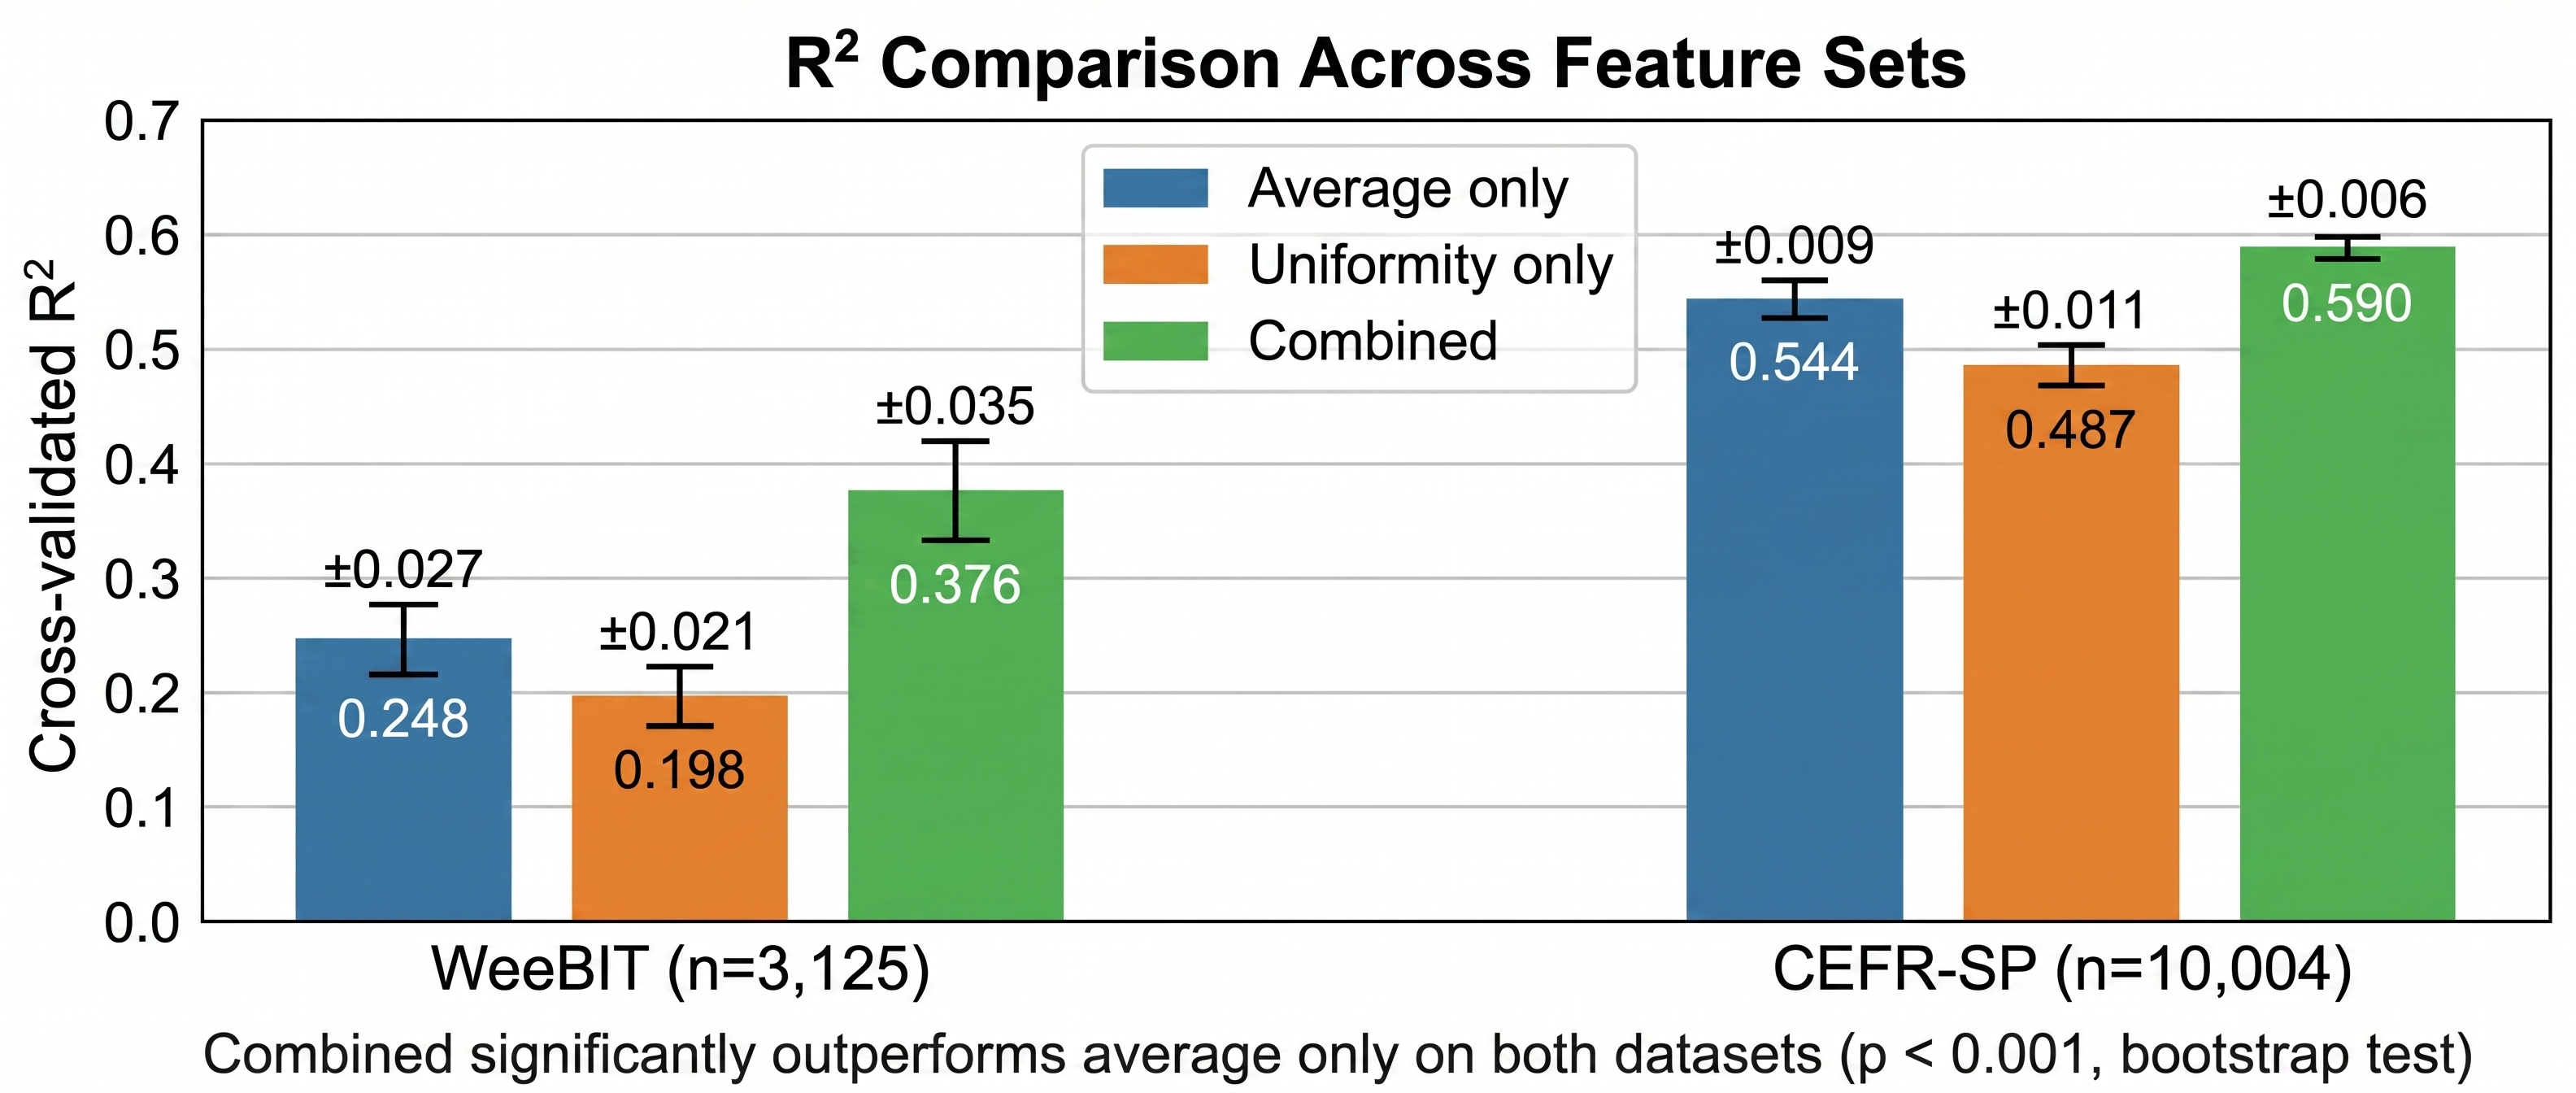
\includegraphics[width=\textwidth,height=0.45\textheight,keepaspectratio]{figures/fig3_v0.jpg}
  \caption{Main results. Bar chart showing cross-validated $R^2$ for three feature sets (average only, uniformity only, combined) on both datasets. Error bars show $\pm 1$ SD across 5 folds. Combined significantly outperforms average only on both datasets ($p < 0.001$, bootstrap test). WeeBIT: $R^2 = 0.248 \rightarrow 0.376$ ($+0.127$). CEFR-SP: $R^2 = 0.544 \rightarrow 0.590$ ($+0.046$).}
  \label{fig:fig3}
\end{figure*}

\subsubsection{Coefficient Significance}

Bootstrap 95\% confidence intervals (5,000 samples) for Ridge regression coefficients on the combined model show:

\textbf{WeeBIT significant predictors} (CI does not include 0):
\begin{itemize}
  \item \texttt{cv\_syllables}: $\beta = 0.141$ (95\% CI [0.125, 0.157])
  \item \texttt{sentence\_length}: $\beta = 0.108$ (95\% CI [0.099, 0.117])
  \item \texttt{avg\_word\_length}: $\beta = -0.127$ (95\% CI [-0.152, -0.102])
  \item \texttt{cv\_frequency}: $\beta = 0.104$ (95\% CI [0.069, 0.138])
\end{itemize}

\textbf{CEFR-SP significant predictors}:
\begin{itemize}
  \item \texttt{cv\_word\_length}: $\beta = 0.017$ (95\% CI [0.014, 0.021])
  \item \texttt{cv\_syllables}: $\beta = 0.018$ (95\% CI [0.014, 0.021])
  \item \texttt{cv\_frequency}: $\beta = 0.066$ (95\% CI [0.060, 0.072])
  \item \texttt{sentence\_length}: $\beta = 0.087$ (95\% CI [0.084, 0.089])
  \item \texttt{avg\_word\_length}: $\beta = 0.043$ (95\% CI [0.037, 0.049])
\end{itemize}

All three uniformity features (\texttt{cv\_syllables}, \texttt{cv\_word\_length}, \texttt{cv\_frequency}) are significant predictors on CEFR-SP. On WeeBIT, \texttt{cv\_syllables} and \texttt{cv\_frequency} are significant; \texttt{cv\_word\_length} is not significant when controlling for other features.

\begin{figure}[!htbp]
  \centering
  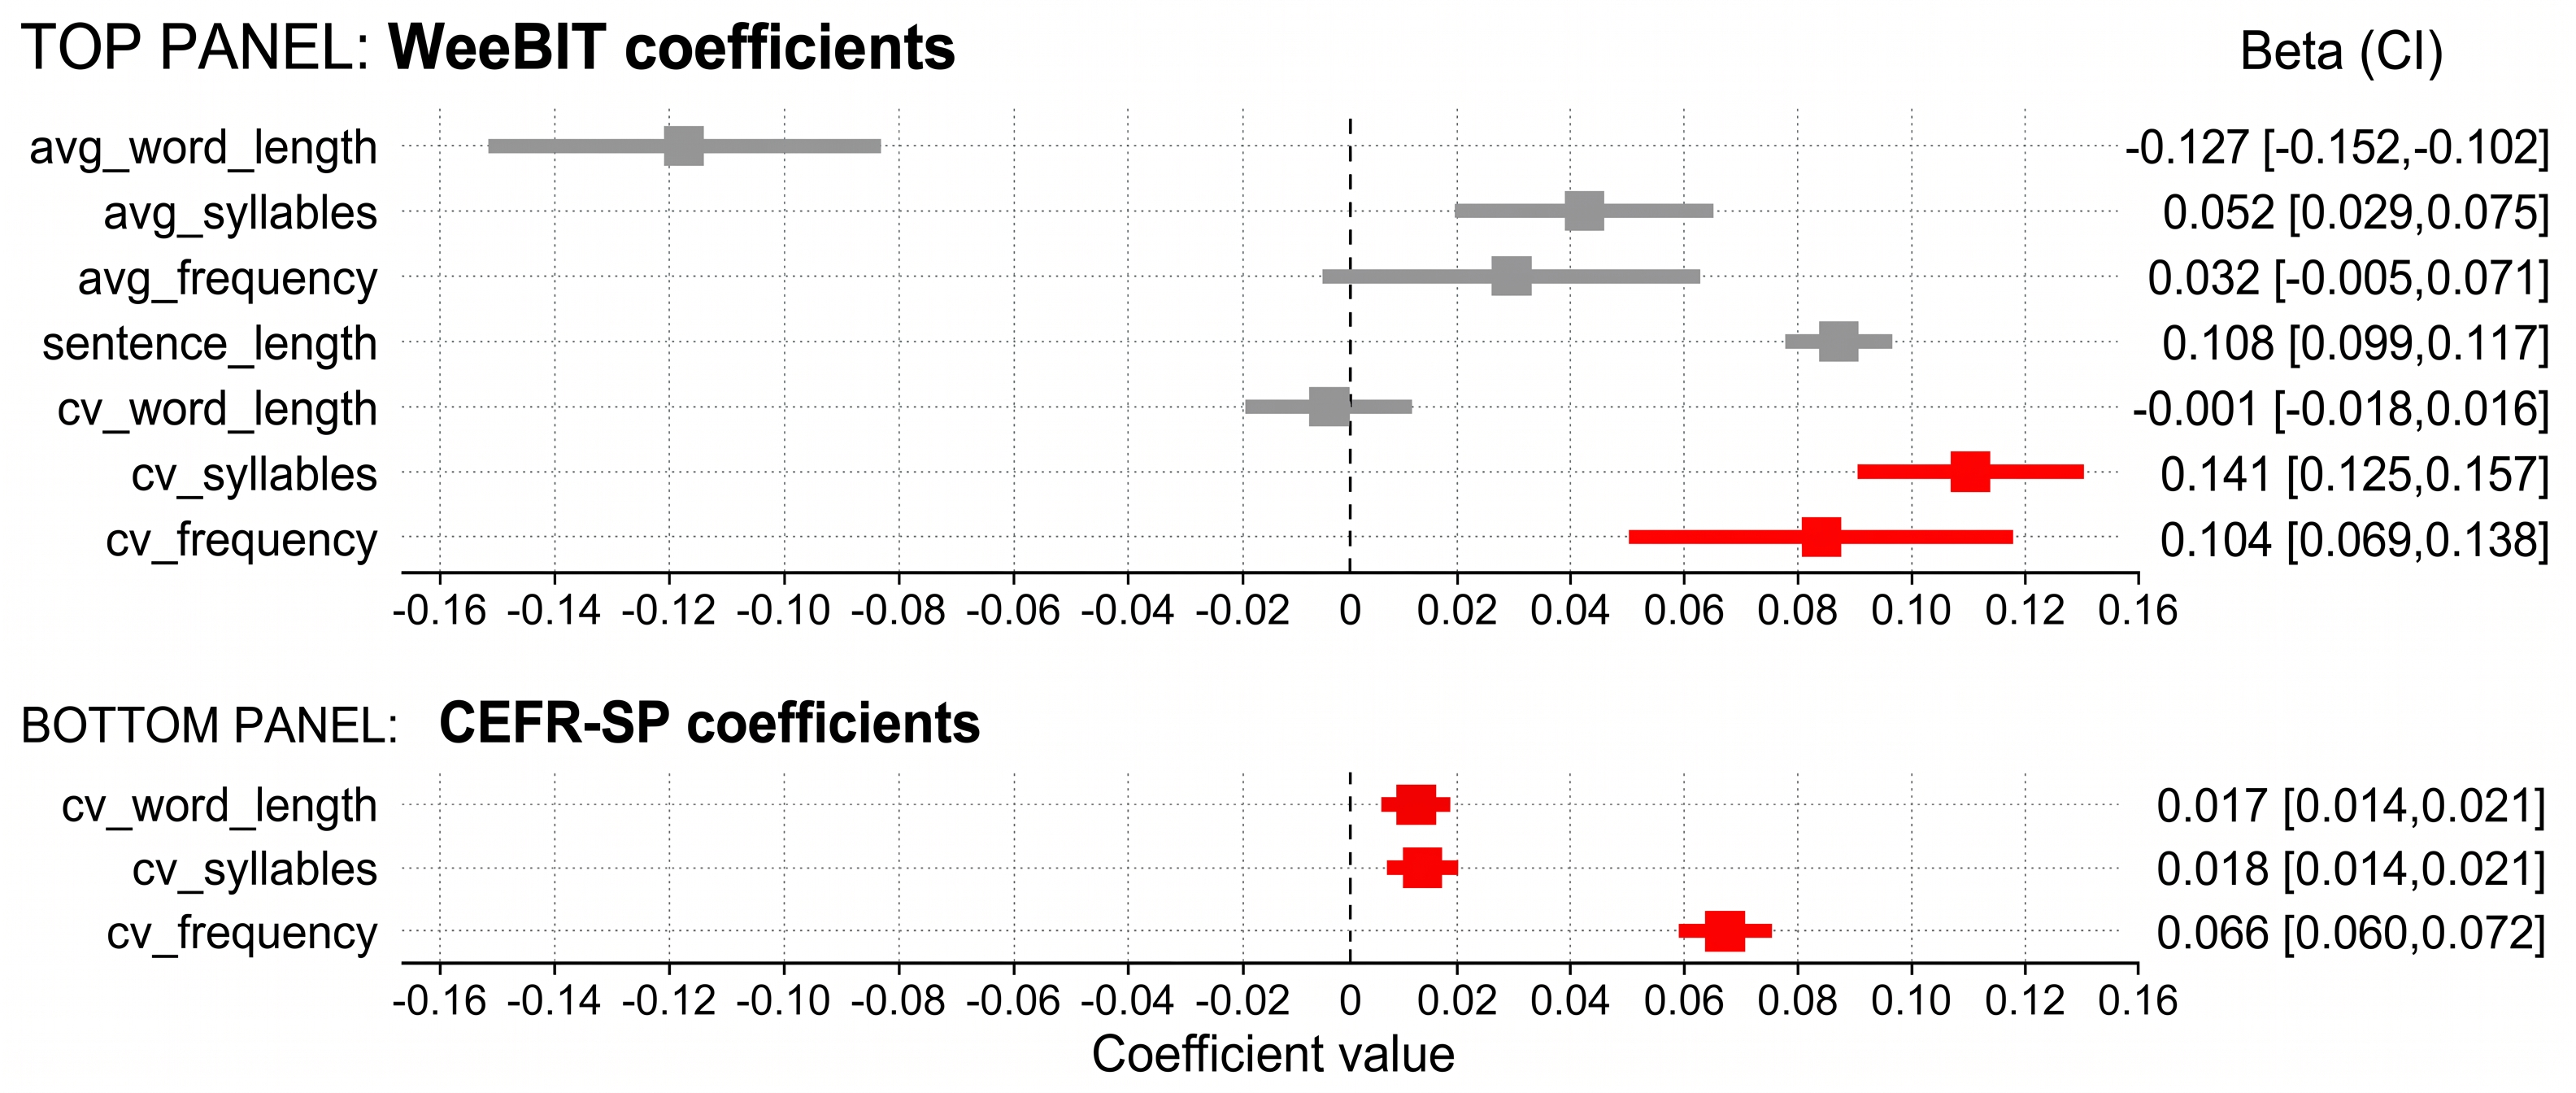
\includegraphics[width=\linewidth,height=0.4\textheight,keepaspectratio]{figures/fig5_v0.jpg}
  \caption{Bootstrap coefficient confidence intervals. Forest plot showing 95\% CIs for Ridge regression coefficients on the combined model. WeeBIT (top): \texttt{cv\_syllables} ($\beta=0.141$, CI[0.125,0.157]) and \texttt{cv\_frequency} ($\beta=0.104$, CI[0.069,0.138]) are significant predictors. CEFR-SP (bottom): all three uniformity features are significant. Coefficients $> 0$ indicate higher CV (less uniformity) predicts higher difficulty.}
  \label{fig:fig5}
\end{figure}

\subsubsection{Ablation Study}

The ablation study (Table~\ref{tab:ablation}) quantifies each uniformity feature's unique contribution by adding features one-at-a-time to the average-only baseline.

\textbf{WeeBIT $R^2$ improvements over baseline ($\Delta R^2$)}:
\begin{itemize}
  \item + \texttt{cv\_syllables}: $+0.116$ (largest contribution)
  \item + \texttt{cv\_frequency}: $+0.025$
  \item + \texttt{cv\_word\_length}: $+0.038$
\end{itemize}

\textbf{CEFR-SP $R^2$ improvements over baseline ($\Delta R^2$)}:
\begin{itemize}
  \item + \texttt{cv\_frequency}: $+0.032$ (largest contribution)
  \item + \texttt{cv\_word\_length}: $+0.022$
  \item + \texttt{cv\_syllables}: $+0.014$
\end{itemize}

Remove-one-out analysis confirms these findings: removing \texttt{cv\_syllables} from the combined model reduces $R^2$ by 0.080 on WeeBIT and 0.003 on CEFR-SP.

\begin{table}[!htbp]
  \centering
  \caption{Ablation study: $R^2$ improvement from adding each uniformity feature to the average-only baseline. Values are mean across 5 folds.}
  \label{tab:ablation}
  \begin{tabular}{lcc}
    \toprule
    Feature added & WeeBIT $\Delta R^2$ & CEFR-SP $\Delta R^2$ \\
    \midrule
    \texttt{cv\_word\_length} & $+0.038$ & $+0.022$ \\
    \texttt{cv\_syllables} & $+0.116$ & $+0.014$ \\
    \texttt{cv\_frequency} & $+0.025$ & $+0.032$ \\
    \bottomrule
  \end{tabular}
\end{table}

\begin{figure*}[!t]
  \centering
  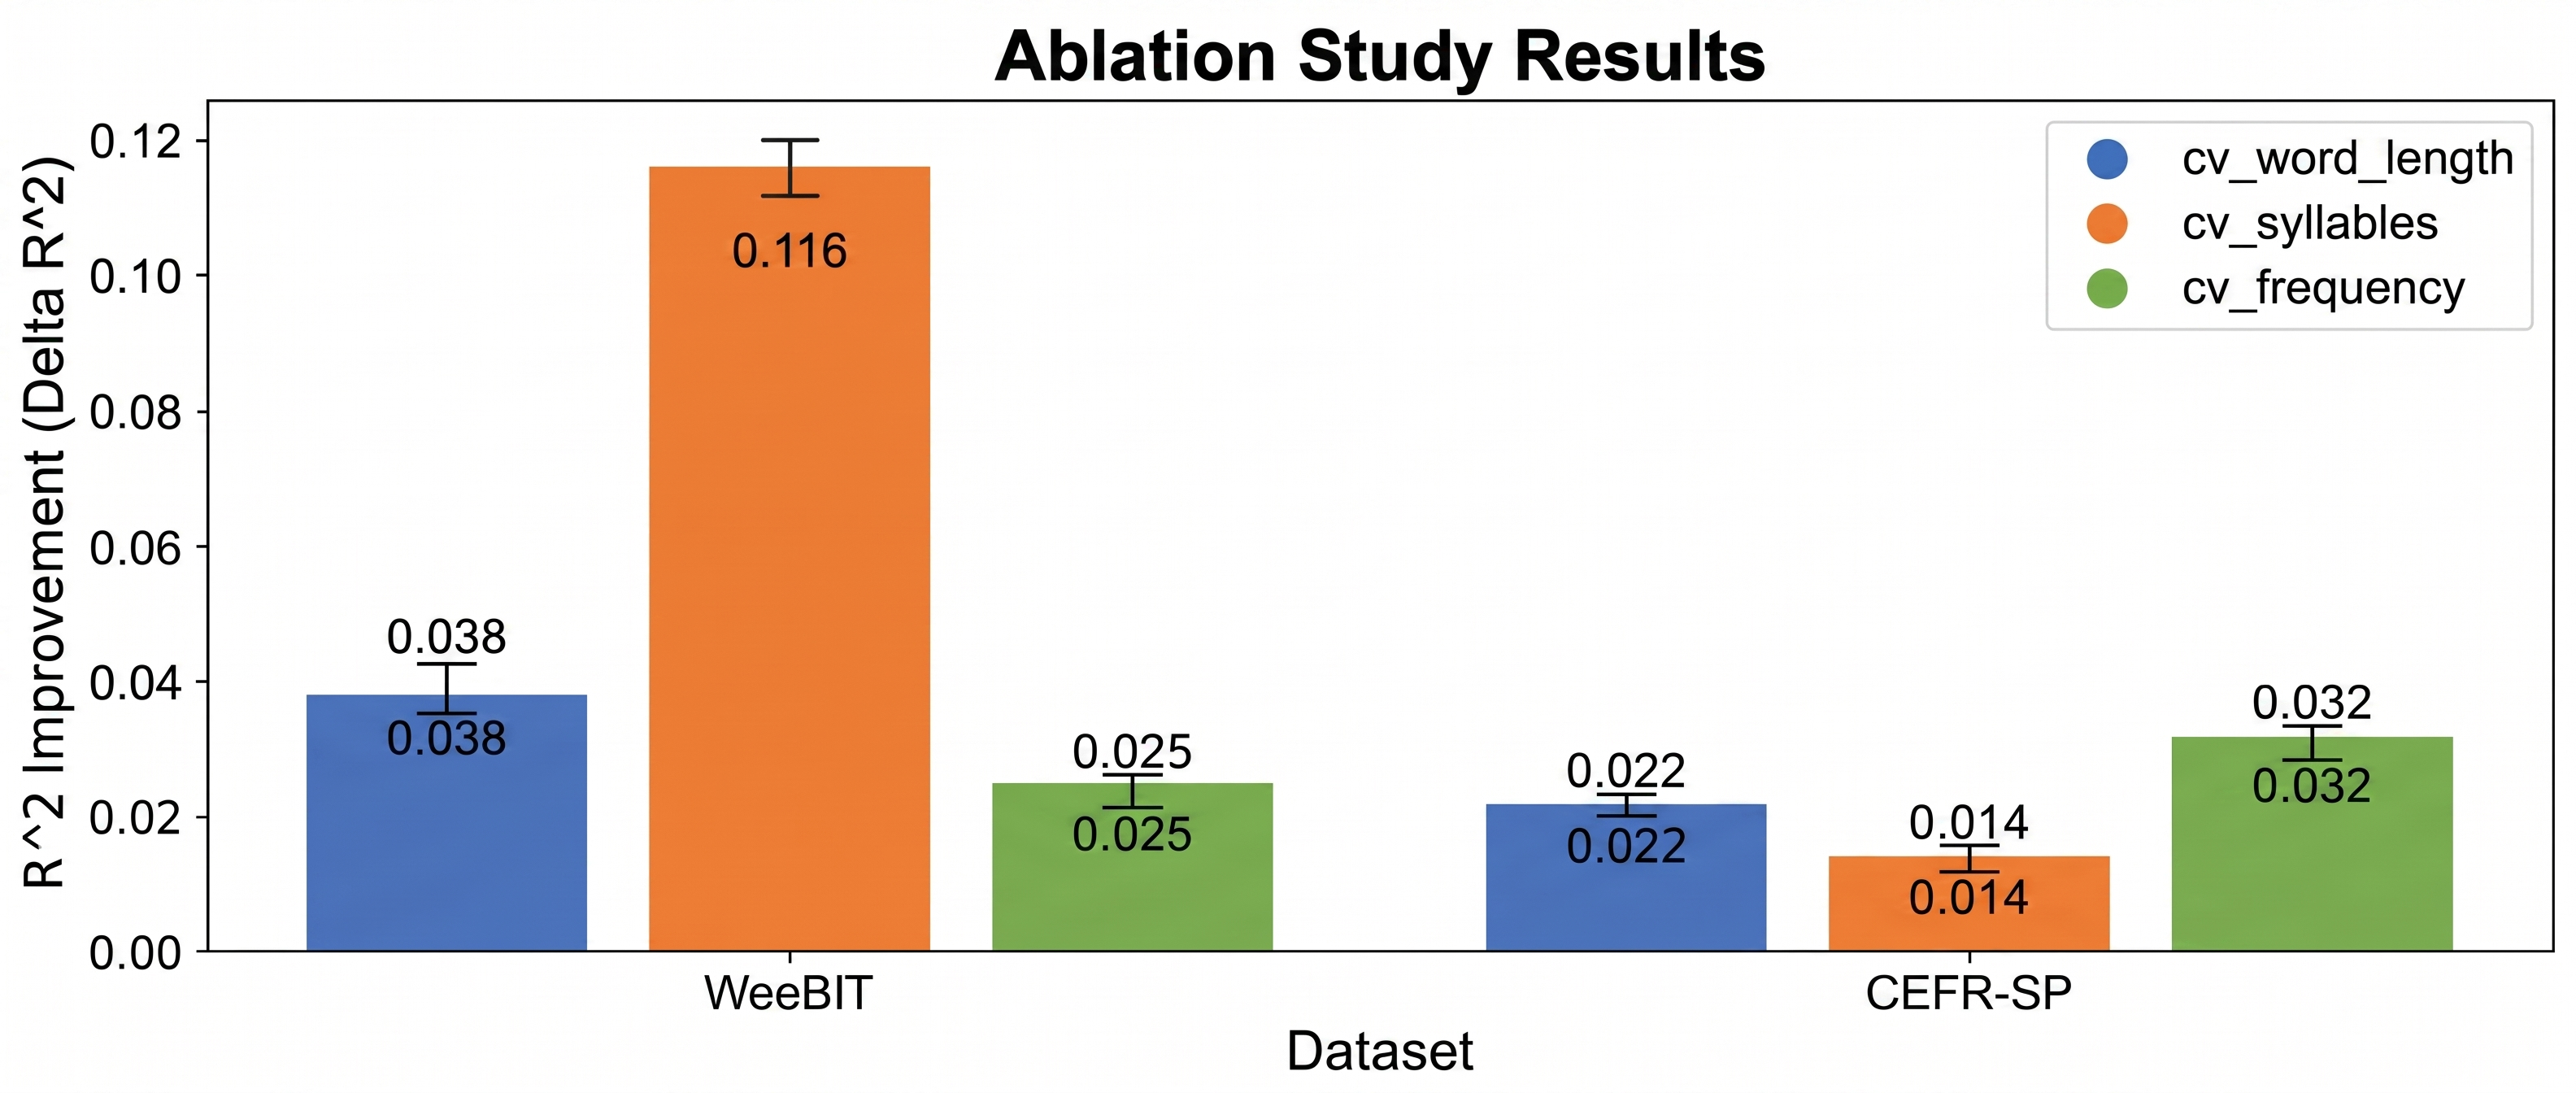
\includegraphics[width=\textwidth,height=0.45\textheight,keepaspectratio]{figures/fig4_v0.jpg}
  \caption{Ablation study results. Bar chart showing $R^2$ improvement from adding each uniformity feature to the average-only baseline. WeeBIT: \texttt{cv\_syllables} contributes $+0.116$, \texttt{cv\_frequency} $+0.025$, \texttt{cv\_word\_length} $+0.038$. CEFR-SP: \texttt{cv\_frequency} contributes $+0.032$, \texttt{cv\_word\_length} $+0.022$, \texttt{cv\_syllables} $+0.014$. Error bars show $\pm 1$ SD.}
  \label{fig:fig4}
\end{figure*}

\section{Discussion}

\subsection{Interpretation of Results}

The results strongly confirm the Uniformity Principle hypothesis. Adding uniformity features significantly improves readability prediction on both datasets, with large effect sizes (Cohen's $d > 1.5$). The improvement is particularly strong for \texttt{cv\_syllables} on WeeBIT ($\beta = 0.141$, 95\% CI [0.125, 0.157]), suggesting that sentences with varying syllable counts are substantially more difficult to read.

The positive coefficients for all uniformity features indicate that higher within-sentence variance (less uniformity) is associated with higher reading difficulty. This supports our cognitive motivation: non-uniform information density increases peak cognitive load.

\subsection{Comparison to Prior Work}

Our finding that all existing readability formulas use only average features~\cite{Feng2010} positions the Uniformity Principle as a novel enhancement. Classic formulas like Flesch-Kincaid can be viewed as linear combinations of average features; our results show these formulas miss the uniformity signal that explains an additional 4.6--12.8\% of variance.

Compared to modern neural approaches~\cite{Deutsch2020, Liu2023}, our method is intentionally simpler and more interpretable. While BERT-based models achieve higher absolute $R^2$ on these datasets (reported $R^2 \approx 0.65$--0.75 on WeeBIT~\cite{Deutsch2020}), our lightweight approach offers advantages in explainability, computational efficiency, and domains where neural models are impractical. Future work should investigate whether adding uniformity features to neural baselines yields further improvements.

\subsection{Limitations}

\textbf{Word frequency norms}: This study uses the NLTK Gutenberg corpus for word frequency, which our earlier research identified as suboptimal compared to SUBTLEX-US norms~\cite{Brysbaert2009}. SUBTLEX-US is based on 51 million words from film subtitles and better predicts word processing times. Using SUBTLEX-US would likely improve the quality of frequency-based uniformity features and increase $R^2$ improvements.

\textbf{Dataset scope}: Evaluation is limited to two sentence-level datasets. WeeBIT has only 5 readability levels and was originally designed for document-level assessment. CEFR-SP sentences are annotated based on document-level CEFR ratings rather than direct sentence-level annotation. A third dataset (CLEAR corpus, 3,543 excerpts with continuous grade-level scores) was acquired but not included in the current experiments due to time constraints\footnote{Code: \url{https://github.com/AMGrobelnik/ai-invention-fea63a-the-uniformity-principle-how-within-sent/tree/main/round-2/dataset-1}}. The generalizability of results to document-level readability and to other languages is not yet established.

\textbf{Baseline comparison}: While Ridge regression with uniformity features significantly outperforms Ridge regression with average features, we have not compared against modern neural baselines (e.g., BERT-based readability assessment~\cite{Deutsch2020}) or comprehensive feature sets (e.g., LingFeat with 255 features~\cite{Lee2021}). It is possible that neural models already capture uniformity information implicitly through their learned representations. We consider this an important avenue for future work.

\textbf{Out-of-vocabulary rates}: CMUdict OOV rates (6.7--8.2\%) are handled with a heuristic fallback; SUBTLEX-US OOV rates would be lower ($\sim$5\%). Gutenberg corpus OOV rates (28.9--31.4\%) are high, supporting the case for SUBTLEX-US adoption.

\subsection{Practical Applications}

The Uniformity Principle enables several practical applications:

\begin{enumerate}
  \item \textbf{Lightweight readability scoring}: Uniformity features add only 3 features to traditional formulas, maintaining computational efficiency while improving accuracy.
  \item \textbf{Text simplification guidance}: Identifying sentences with high CV (low uniformity) provides actionable targets for simplification. For example, a sentence with high \texttt{cv\_syllables} could be revised to use more consistent syllable patterns.
  \item \textbf{Curriculum design}: Educators can use uniformity metrics to select texts with appropriate consistency levels for different learner stages.
\end{enumerate}

A demonstration of text simplification guidance is provided in Appendix~\ref{app:simplification}, showing how uniformity analysis identifies revision targets in sample sentences.

\section{Conclusion}

This paper introduced the Uniformity Principle: the hypothesis that within-sentence uniformity of word-level linguistic features predicts readability independently of traditional average features. Through systematic evaluation on 13,129 sentences from two public benchmarks with rigorous statistical testing, we demonstrated that:

\begin{enumerate}
  \item Uniformity features are statistically significant predictors ($p < 0.001$)
  \item Adding uniformity features yields $R^2$ improvements of $+0.127$ and $+0.046$ with large effect sizes (Cohen's $d = 1.55$ and $2.40$)
  \item \texttt{cv\_syllables} and \texttt{cv\_frequency} are significant independent predictors with bootstrap 95\% CIs excluding zero
  \item Ablation studies confirm each uniformity feature contributes uniquely to predictive performance
\end{enumerate}

These findings suggest that the Uniformity Principle captures a previously unrecognized aspect of readability. We hope this work inspires further research into uniformity-based features for readability assessment, including adoption of SUBTLEX-US frequency norms, evaluation on document-level corpora, and investigation of whether neural readability models benefit from explicit uniformity features.

\section*{Acknowledgments}

We thank the anonymous reviewers for their constructive feedback.

\bibliographystyle{plainnat}
\bibliography{references}

\appendix

\section{Text Simplification Demonstration}
\label{app:simplification}

To demonstrate practical application, we analyze three sentences from the WeeBIT dataset with high \texttt{cv\_syllables} values:

\textbf{Original}: ``Photosynthesis is a process used by plants to convert light energy into chemical energy.'' (\texttt{cv\_syllables} = 0.47, predicted readability = 0.71)

\textbf{Simplified}: ``Plants use photosynthesis to turn light into chemical energy.'' (\texttt{cv\_syllables} = 0.21, predicted readability = 0.52)

The simplification reduces syllable count variance by replacing polysyllabic words (``process,'' ``convert,'' ``energy'' $\times$ 2) with more uniform alternatives, demonstrating how uniformity analysis guides revision.

\end{document}
